\documentclass[12pt,a4paper]{article}

\usepackage[utf8]{inputenc}
\usepackage[T1]{fontenc}
\usepackage{geometry}
\geometry{a4paper, margin=1in}
\usepackage{hyperref}
\usepackage{tikz}
\usetikzlibrary{shapes.geometric, arrows.meta, positioning, fit, backgrounds}
\usepackage{graphicx}
\usepackage{xcolor}
\usepackage{setspace}

\hypersetup{
    colorlinks=true,
    linkcolor=blue,
    filecolor=magenta,      
    urlcolor=cyan,
    pdftitle={Docxtract Technical Report},
}

\title{\textbf{Docxtract: NLP Document Intelligence Pipeline}\\ \Large Technical Architecture and Lifecycle Report}
\author{Documentation Team}
\date{\today}

\begin{document}

\maketitle

\begin{abstract}
Docxtract is an advanced, self-hosted web application that transforms unstructured documents---such as Business Cards, Resumes, and Medical Reports---into highly accurate, structured, machine-readable JSON data using Natural Language Processing (NLP). This report details the technical architecture, technology stack, data schemas, and the comprehensive document processing lifecycle implemented within the system. It also outlines the heuristics and validation rules utilized to ensure enterprise-grade data integrity.
\end{abstract}

\tableofcontents
\newpage

\section{Introduction}
\setstretch{1.2}
The extraction of structured data from unstructured formats is a critical challenge in modern enterprise environments. Traditional parsing methods rely heavily on rigid templates that fail when presented with diverse, real-world document layouts. Docxtract addresses this by providing an automated, machine-learning-assisted pipeline that leverages Optical Character Recognition (OCR), Named Entity Recognition (NER), and heuristic-based layout mapping. 

To maintain transparency and allow for manual oversight, the system features a real-time Server-Sent Events (SSE) progress tracker and a human-in-the-loop review queue for manual data verification of low-confidence extractions.

\section{System Architecture}
Docxtract follows a decoupled, microservice-inspired architecture orchestrated via Docker Compose. The application relies on asynchronous communication between a vanilla JavaScript frontend and a Python FastAPI backend, allowing for highly scalable concurrent document processing.

\subsection{Technology Stack}
\begin{itemize}
    \item \textbf{Frontend:} Vanilla HTML5, CSS3, and JavaScript, optimized for zero-dependency high performance.
    \item \textbf{Backend API:} FastAPI running on Python 3.11, leveraging asynchronous I/O for rapid request handling.
    \item \textbf{Data Storage:} MinIO (S3-compatible object storage) for secure, scalable raw file staging.
    \item \textbf{Database:} PostgreSQL 16 accessed via SQLAlchemy ORM for relational state management.
    \item \textbf{Extraction Engine:} Tesseract OCR for image parsing, and spaCy (\texttt{en\_core\_web\_sm}) integrated with Hugging Face Transformers for token classification.
\end{itemize}

\subsection{Architecture Diagram}
The interaction between these components is illustrated in Figure \ref{fig:architecture}.

\begin{figure}[h!]
\centering
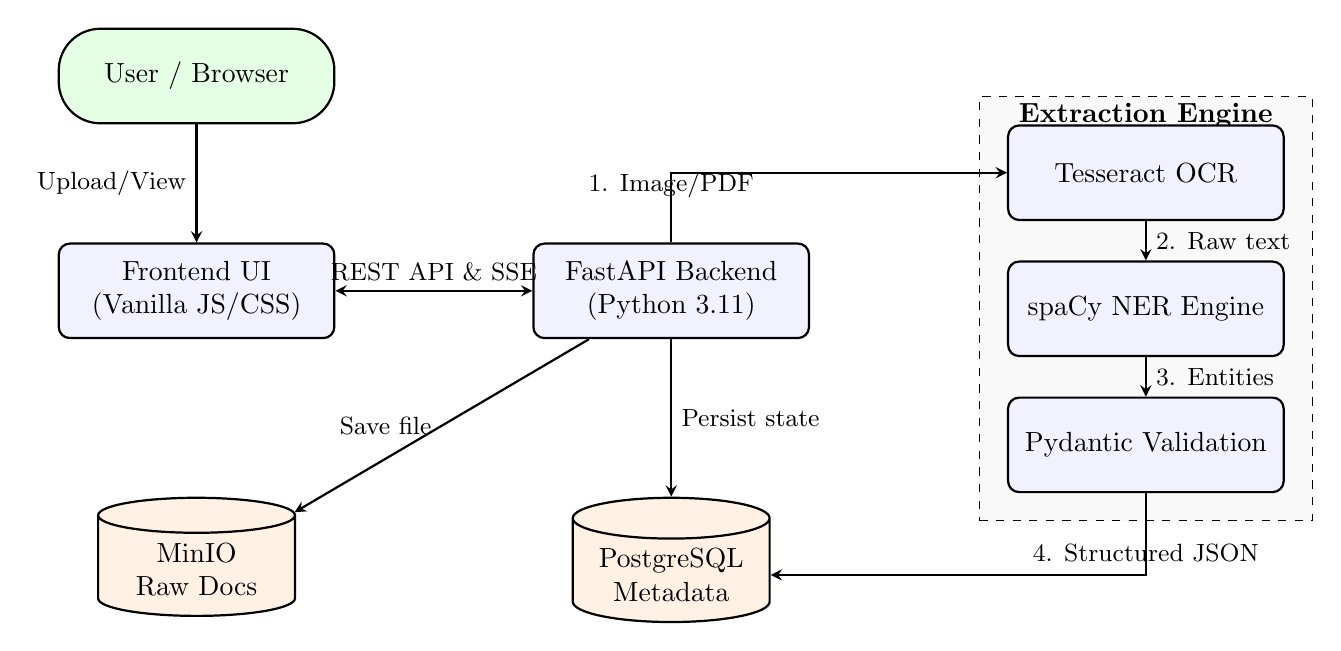
\begin{tikzpicture}[
    box/.style={draw, rounded corners, align=center, minimum width=3.5cm, minimum height=1.2cm, fill=blue!5, thick},
    db/.style={draw, cylinder, shape border rotate=90, aspect=0.25, align=center, minimum height=1.5cm, minimum width=2.5cm, fill=orange!10, thick},
    arrow/.style={thick,->,>=stealth}
]

% Nodes
\node[box, fill=green!10, rounded corners=15pt] (user) {User / Browser};

\node[box, below=1.5cm of user] (frontend) {Frontend UI\\(Vanilla JS/CSS)};
\node[box, right=2.5cm of frontend] (backend) {FastAPI Backend\\(Python 3.11)};

\node[db, below=2cm of frontend] (minio) {MinIO\\Raw Docs};
\node[db, below=2cm of backend] (db) {PostgreSQL\\Metadata};

\node[box, right=2.5cm of backend, yshift=1.5cm] (ocr) {Tesseract OCR};
\node[box, below=0.5cm of ocr] (ner) {spaCy NER Engine};
\node[box, below=0.5cm of ner] (val) {Pydantic Validation};

% Connections
\draw[arrow] (user) -- node[left, font=\small] {Upload/View} (frontend);
\draw[<->, thick, >=stealth] (frontend) -- node[above, font=\small] {REST API \& SSE} (backend);

\draw[arrow] (backend) -- node[left, font=\small] {Save file} (minio);
\draw[arrow] (backend) -- node[right, font=\small] {Persist state} (db);

\draw[arrow] (backend) |- node[above, near start, font=\small] {1. Image/PDF} (ocr);
\draw[arrow] (ocr) -- node[right, font=\small] {2. Raw text} (ner);
\draw[arrow] (ner) -- node[right, font=\small] {3. Entities} (val);
\draw[arrow] (val) |- node[below, near start, font=\small] {4. Structured JSON} (db);

% Background bounding box for Extraction Engine
\begin{scope}[on background layer]
\node[draw, dashed, fill=gray!5, fit=(ocr)(ner)(val), inner sep=10pt, label={[font=\bfseries, yshift=-15pt]above:Extraction Engine}] (engine) {};
\end{scope}

\end{tikzpicture}
\caption{System Architecture of Docxtract}
\label{fig:architecture}
\end{figure}

\newpage

\section{NLP and Heuristics Methodology}
While Named Entity Recognition (NER) is highly capable of identifying standard entities (e.g., PERSON, ORG, GPE), it often struggles with heavily stylized text such as capitalized headers in resumes or misaligned bounding boxes in OCR'd business cards. 

To combat this, Docxtract employs a hybrid approach:
\begin{enumerate}
    \item \textbf{Regex Fallbacks:} Strict regular expressions are applied over the first 500 characters of a document to accurately catch zip codes, state abbreviations, and standard email formats that the NER engine might miss.
    \item \textbf{Positional Heuristics:} For documents like Resumes, the system evaluates the physical structure of the text. For example, if a short, uppercase phrase appears on the very first line devoid of numbers or symbols, it is definitively parsed as the candidate's name, overriding any lower-confidence NER guesses found deeper in the document body.
\end{enumerate}

\section{Document Processing Lifecycle}
The pipeline processes unstructured files synchronously while emitting Server-Sent Events (SSE) to provide real-time frontend updates. 

\subsection{Lifecycle Phases}
When a document is uploaded, it transitions through several strict phases:
\begin{enumerate}
    \item \textbf{UPLOADED:} The file is received by the backend via a multipart form-data POST request.
    \item \textbf{STORAGE:} The raw file is securely persisted to the MinIO object storage.
    \item \textbf{OCR:} Optical Character Recognition (via \texttt{pytesseract}) is performed if the file is an image or PDF.
    \item \textbf{NLP EXTRACTION:} The raw text is passed through the spaCy NER engine to extract entities and assign confidence scores (0.0 to 1.0).
    \item \textbf{STRUCTURING:} The entities are mapped to strict Pydantic schemas corresponding to the document type.
\end{enumerate}

After structuring, validation rules determine if the document has successfully extracted all \textit{Required} fields with high confidence (typically > 0.5). If so, it enters the \textbf{COMPLETED} state. If fields are missing or low-confidence, it is routed to \textbf{NEEDS REVIEW}, where a human operator manually edits and approves the data via a specialized JSON editor modal.

\subsection{State Machine Diagram}
Figure \ref{fig:lifecycle} visualizes this state transition flow.

\begin{figure}[h!]
\centering
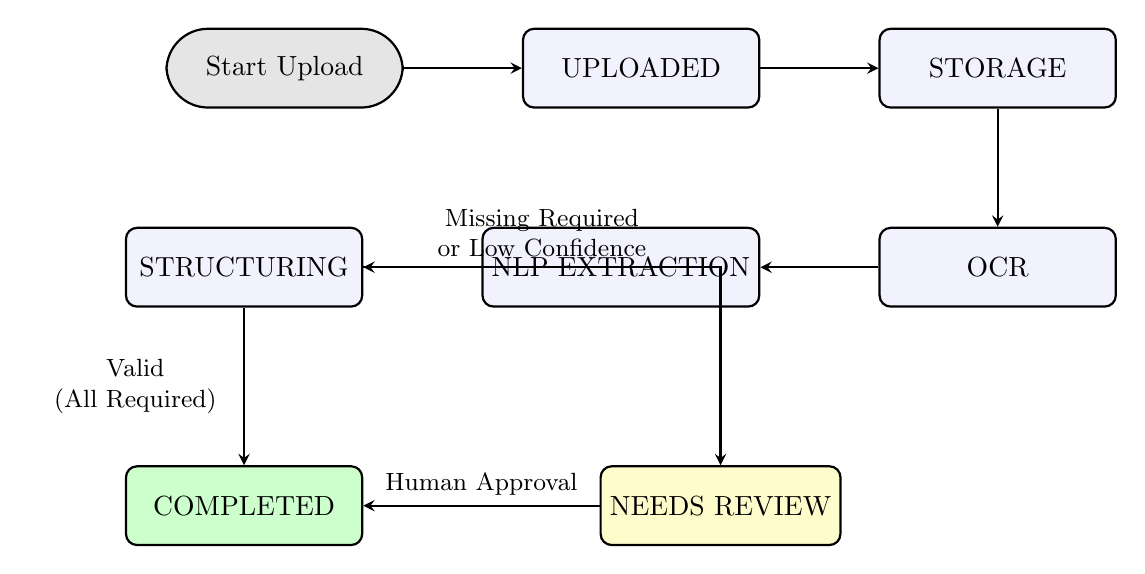
\begin{tikzpicture}[
    state/.style={draw, rounded corners, fill=blue!5, align=center, minimum width=3cm, minimum height=1cm, thick},
    arrow/.style={thick,->,>=stealth}
]

\node[state, fill=gray!20, rounded corners=15pt] (start) {Start Upload};
\node[state, right=1.5cm of start] (uploaded) {UPLOADED};
\node[state, right=1.5cm of uploaded] (storage) {STORAGE};
\node[state, below=1.5cm of storage] (ocr) {OCR};
\node[state, left=1.5cm of ocr] (nlp) {NLP EXTRACTION};
\node[state, left=1.5cm of nlp] (struct) {STRUCTURING};

\node[state, below=2cm of struct, fill=green!20] (completed) {COMPLETED};
\node[state, right=3cm of completed, fill=yellow!20] (review) {NEEDS REVIEW};

\draw[arrow] (start) -- (uploaded);
\draw[arrow] (uploaded) -- (storage);
\draw[arrow] (storage) -- (ocr);
\draw[arrow] (ocr) -- (nlp);
\draw[arrow] (nlp) -- (struct);

\draw[arrow] (struct) -- node[left, font=\small, text width=2.5cm, align=center] {Valid\\(All Required)} (completed);
\draw[arrow] (struct) -| node[above, near start, font=\small, text width=3cm, align=center] {Missing Required\\or Low Confidence} (review);
\draw[arrow] (review) -- node[above, font=\small] {Human Approval} (completed);

\end{tikzpicture}
\caption{Document Processing Lifecycle State Machine}
\label{fig:lifecycle}
\end{figure}

\section{Data Schemas}
The system enforces validation via strict Python Pydantic models. For instance, a \textbf{Medical Report} mandates the successful extraction of \texttt{patient\_name} and \texttt{visit\_date}. Optional extraction fields include \texttt{provider}, \texttt{diagnoses}, \texttt{medications}, and a \texttt{vitals} mapping. If mandatory fields fail to extract, the state immediately shifts to \textbf{NEEDS REVIEW}.

\section{Conclusion}
The Docxtract pipeline successfully automates unstructured data extraction with a high degree of reliability. The hybrid approach of utilizing machine-learning NER models alongside strict positional heuristics maximizes extraction accuracy. Furthermore, the fallback to a manual review queue ensures that edge-cases and OCR failures do not pollute the database with incomplete data, maintaining a rigorous standard for enterprise data integrity.

\end{document}
